\documentclass[tikz,border=7pt]{standalone}
\usepackage[T1]{fontenc}
\usepackage[utf8]{inputenc}
\usetikzlibrary{positioning,arrows.meta}
\begin{document}
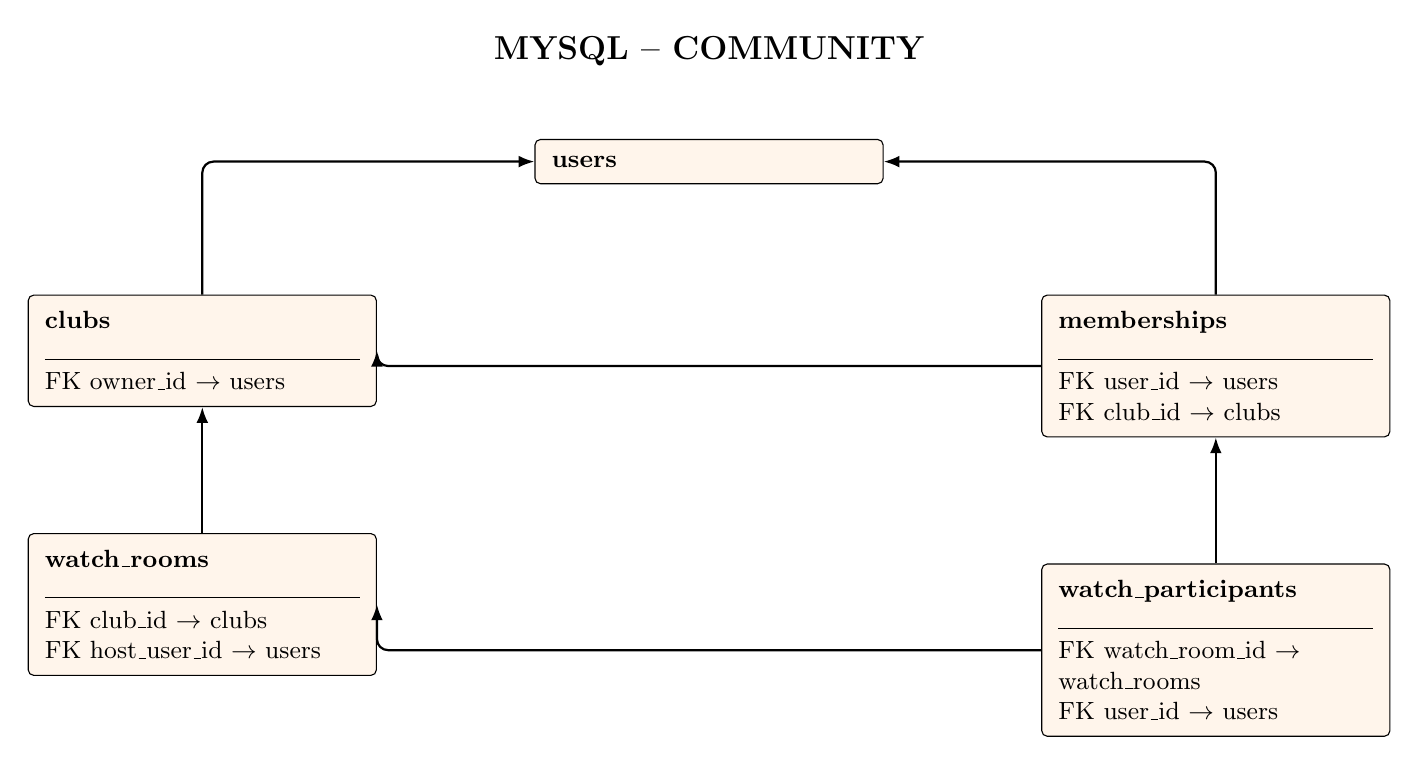
\begin{tikzpicture}[font=\small, entity/.style={draw, rounded corners=2pt, align=left, text width=4cm, inner sep=6pt, fill=orange!8}, heading/.style={font=\bfseries\large}, rel/.style={-{Latex[length=2mm]}, rounded corners, thick}]
\node[heading] (title) {MYSQL -- COMMUNITY};
\node[entity, below=8mm of title] (users) {\textbf{users}};
\node[entity, below left=14mm and 20mm of users] (clubs) {\textbf{clubs}\\\rule{4cm}{0.3pt}\\FK owner\_id $\rightarrow$ users};
\node[entity, below right=14mm and 20mm of users] (memberships) {\textbf{memberships}\\\rule{4cm}{0.3pt}\\FK user\_id $\rightarrow$ users\\FK club\_id $\rightarrow$ clubs};
\node[entity, below=16mm of clubs] (rooms) {\textbf{watch\_rooms}\\\rule{4cm}{0.3pt}\\FK club\_id $\rightarrow$ clubs\\FK host\_user\_id $\rightarrow$ users};
\node[entity, below=16mm of memberships] (participants) {\textbf{watch\_participants}\\\rule{4cm}{0.3pt}\\FK watch\_room\_id $\rightarrow$ watch\_rooms\\FK user\_id $\rightarrow$ users};
\draw[rel] (clubs.north) |- (users.west);
\draw[rel] (memberships.north) |- (users.east);
\draw[rel] (memberships.west) -| (clubs.east);
\draw[rel] (rooms.north) -- (clubs.south);
\draw[rel] (participants.north) -- (memberships.south);
\draw[rel] (participants.west) -| (rooms.east);
\end{tikzpicture}
\end{document}
